\documentclass[12pt]{article}
\usepackage[margin=1in]{geometry} 
\usepackage{amsmath, amsthm, amssymb, scrextend, cancel, mathtools}
\usepackage{tikz-qtree}
\begin{document}
    \section*{1 Study Group}
    \color{blue}
    Lakshya Nagal, SID: 3037935253 
    \color{black}
    \newpage
    \section*{2 Course Policies}
    \begin{enumerate}
        \item[\textbf{(a)}]
        \color{blue}
            \begin{itemize}
                \item Midterm 1: Monday, 2/26/2024, 7:00 PM - 9:00 PM
                \item Midterm 2: Tuesday, 4/2/2024, 7:00 PM - 9:00 PM
                \item Final: Friday, 5/10/2024, 7:00 PM - 10:00 PM (Group 20)
            \end{itemize}
        \color{black}
        \item[\textbf{(b)}]
        \color{blue}
            It is recommended that homework be finished by 10:00 PM.
        \color{black}
        \item[\textbf{(c)}]
        \color{blue}
            Nothing, since there are no exeptions after the deadline of 11:59 PM; however, you may
            use one of your two drops.
        \color{black}
        \item[\textbf{(d)}]
        \color{blue}
            Ed is the primary source of communication between students and staff.
        \color{black}
        \item[\textbf{(e)}]  
        \color{blue}
            I have read and understood the course syllabus and policies.
    \end{enumerate}
    \newpage
    \section*{3 Understanding Academic Dishonesty}
    \begin{enumerate}
        \color{black}
        \item[\textbf{(a)}] 
        \color{blue}
        Not okay.
        \color{black}
        \item[\textbf{(b)}] 
        \color{blue}
        Not okay.
        \color{black}
        \item[\textbf{(c)}] 
        \color{blue}
        Not okay.
        \color{black}
        \item[\textbf{(d)}] 
        \color{blue}
        Okay.  
    \end{enumerate}
    \newpage
    \section*{4 Math Potpourri}
    \begin{enumerate}
        \item[\textbf{(a)}] Simplify the following expressions into a single logarithm (i.e. in the form $\log_a(b)$:
            \begin{enumerate} 
                \item[(i)]
                \color{blue}
                    \begin{align*}
                        \frac{\ln(x)}{\ln(y)} = \frac{\log_e(x)}{\log_e(y)} = \boxed{\log_y(x)}
                    \end{align*}
                \color{black}
                \item[(ii)]
                \color{blue}
                    \begin{align*}
                        \ln(x) + \ln(y) = \boxed{\ln(x \cdot y)}
                    \end{align*}
                \color{black}
                \item[(iii)]
                \color{blue}
                    \begin{align*}
                        \ln(x) - \ln(y) = \boxed{\ln\left(\frac{x}{y}\right)}
                    \end{align*}
                \color{black}
                \item[(iv)]
                \color{blue}
                    \begin{align*}
                        170\ln(x) = \boxed{\ln(x^{170})}
                    \end{align*}
                \color{black}
            \end{enumerate}
        \item[\textbf{(b)}] Give a simple proof for each of the following identities:
            \begin{enumerate}
                \item[(a)]
                \color{blue}
                    \begin{align*}
                        x^{\log_{\frac{1}{x}}(y)} &= \frac{1}{\frac{1}{x^{\log_{\frac{1}{x}(y)}}}} \\
                        &= \frac{1}{\left(\frac{1}{x}\right)^{\log_{\frac{1}{x}}(y)}} \\
                        &= \frac{1}{y}
                    \end{align*}
                \color{black}
                \item[(b)]
                \color{blue}
                    \begin{align*}
                        \sum_{i=1}^{n}i &= 1 + 2 + 3 + \cdots + (n-1) + n \\
                        &= (1 + n) + (2 + (n-1)) + (3 + (n-2)) + \cdots \\
                        &= (n + 1) + (n + 1) + (n + 1) + \cdots \\
                        &= (n + 1) \cdot \left(\frac{n}{2}\right) \\
                        &= \frac{n(n + 1)}{2}
                   \end{align*}
                \color{black}
                \item[(c)]
                \color{blue}
                   \begin{align*}
                        \text{If r = 1 then...} \\
                        \sum_{k=0}^{n}ar^k = \sum_{k=0}^{n}a = a\sum_{k=0}^{n}1 &= a \cdot (n + 1)\\
                        \text{If r $\ne$ 1 then...} \\
                        \text{Let $x_n = \sum_{k=0}^{n}ar^k$} \\
                        x_n = ar^0 + ar^1 + ar^2 + &\cdots + ar^n \\
                        \text{Multiply both sides}&\text{ by $r$}\\
                        rx_n = ar^1 + ar^2 + ar^3 + &\cdots + ar^{n+1} \\
                        x_n - rx_n = ar^0 - &ar^{n+1} \\
                        x_n(1-r) = a(1-&r^{n+1}) \\
                        \sum_{k=0}^{n}ar^k = \frac{a(1-r^{n+1})}{1-r}& \\ \\
                     \end{align*}
                \color{black}
            \end{enumerate}
    \end{enumerate}
    \newpage
    \section*{5 Recurrence Relations}
    \begin{enumerate}
        \item[\textbf{(a)}] $T(n) = 2T(n/3) + 5n$ \\
            \tikzset{every tree node/.style={minimum width=1em,draw,circle},
            blank/.style={draw=none},
            edge from parent/.style=
            {draw,edge from parent path={(\tikzparentnode) -- (\tikzchildnode)}},
            level distance=1.2cm}
            \color{blue}
            \begin{center}
                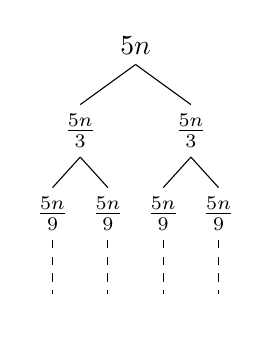
\begin{tikzpicture}
                    \Tree
                    [.$5n$     
                        [.$\frac{5n}{3}$ 
                            \edge[]; 
                                [.$\frac{5n}{9}$
                                \edge[dashed]; {}
                                ]
                            \edge[];
                                [.$\frac{5n}{9}$
                                \edge[dashed]; {}
                                ]
                        ]
                        [.$\frac{5n}{3}$ 
                            \edge[];
                                [.$\frac{5n}{9}$
                                \edge[dashed]; {}
                                ]
                            \edge[];
                                [.$\frac{5n}{9}$
                                \edge[dashed]; {}
                                ]
                        ]
                    ]
                \end{tikzpicture} \\
                Level 1: $5n$ \\
                Level 2: $2 \frac{5n}{3}$ \\
                Level 3: $4 \frac{5n}{9}$\\
                $\vdots$ \\
            \end{center}
            \begin{align*}
                \sum_{k = 0}^{\log_3n} 2^k\cdot\frac{5n}{3^k} &= 5n\sum_{k = 0}^{\log_3n} \left(\frac{2}{3}\right)^k \le \sum_{k=0}^{\infty} \left(\frac{2}{3}\right)^k\\
                &= 5n\left[\left(\frac{2}{3}\right)^0 + \left(\frac{2}{3}\right)^1 + \left(\frac{2}{3}\right)^2 + \cdots)\right] \\
                &= 5n\left[\frac{1}{1-\frac{2}{3}}\right]\\
                &= 15n\\
                &=\boxed{\Theta(n)} \\
            \end{align*} 
            \newpage
        \color{black}               
        \item[\textbf{(b)}] $T(n) = 169T(n/170) + \Theta(n)$ \\
        \color{blue}
            \begin{center}
                There are 169 branches for every node. At the $k^{th}$ level \\we do $\frac{169^kn}{170^k}$ work and there are 
                $\log_{170}n$ levels in the tree.
            \end{center}
            \begin{align*}
                \sum_{k = 0}^{\log_{170}n} \frac{169^kn}{170^k} &= n\left[\sum_{k = 0}^{\log_{170}n}\left(\frac{169}{170}\right)^k\right] \le n\left[\sum_{k=0}^{\infty}\left(\frac{169}{170}\right)^k\right]\\
                &=n\left[\left(\frac{169}{170}\right)^0+\left(\frac{169}{170}\right)^1+\left(\frac{169}{170}\right)^2+\cdots\right] \\
                &=n\left[\frac{1}{1-\frac{169}{170}}\right] \\
                &=\boxed{\Theta\left(n\right)}
            \end{align*}
        \color{black}
        \item[\textbf{(c)}] An algorithm A takes $\Theta(n^2)$ time to partition the input into 5 sub-problems of size $n/5$. Describe the recurrence
        relation for the run-time $T(n)$ of $\mathcal{A}$ and find its asymptotic order of growth. \\
            \tikzset{every tree node/.style={minimum width=0.0em,draw,circle},
            blank/.style={draw=none},
            edge from parent/.style=
            {draw,edge from parent path={(\tikzparentnode) -- (\tikzchildnode)}},
            level distance=1.5cm}
            \color{blue}
            \begin{center}
                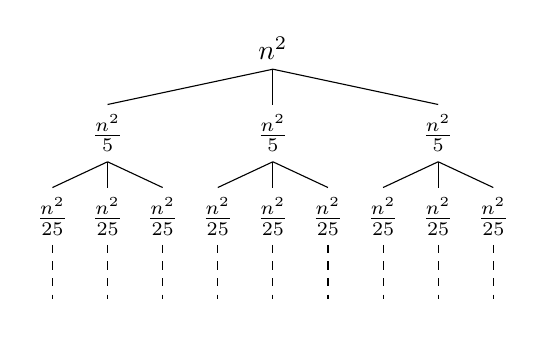
\begin{tikzpicture}
                    \Tree
                    [.$n^2$     
                        [.$\frac{n^2}{5}$ 
                            \edge[];
                            [.$\frac{n^2}{25}$
                                \edge[dashed];
                                [.$$
                                ]
                            ]
                            \edge[];
                            [.$\frac{n^2}{25}$
                                \edge[dashed];
                                [.$$
                                ]
                            ]
                            \edge[];
                            [.$\frac{n^2}{25}$
                            \edge[dashed];
                                [.$$
                                ]
                            ]
                        ]
                        [.$\frac{n^2}{5}$
                            \edge[];
                            [.$\frac{n^2}{25}$
                                \edge[dashed];
                                [.$$
                                ]
                            ]
                            \edge[];
                            [.$\frac{n^2}{25}$
                                \edge[dashed];
                                [.$$
                                ]
                            ]
                            \edge[];
                            [.$\frac{n^2}{25}$
                            \edge[dashed];
                                [.$$
                                ]
                            ]
                        ]
                        [.$\frac{n^2}{5}$ 
                            \edge[];
                            [.$\frac{n^2}{25}$
                                \edge[dashed];
                                [.$$
                                ]
                            ]
                            \edge[];
                            [.$\frac{n^2}{25}$
                                \edge[dashed];
                                [.$$
                                ]
                            ]
                            \edge[];
                            [.$\frac{n^2}{25}$
                            \edge[dashed];
                                [.$$
                                ]
                            ]
                        ]
                    ]
                \end{tikzpicture} \\
                Giving the recurrence relation $\Rightarrow T(n) = 3T (n/5)+ \Theta(n^2)$ \\
            Level 1: $n^2$ work, Level 2: $3\frac{n^2}{5}$ work, Level 3: $9\frac{n^2}{25}$ work, ...
            \end{center}
            \begin{align*}
                \sum_{k = 0}^{\log_5(n)}\frac{3^kn^2}{5^k} &= n^2\sum_{k = 0}^{\log_5(n)}\left(\frac{3}{5}\right)^k \le n^2\sum_{k = 0}^{\infty}\left(\frac{3}{5}\right)^k\\
                &=n^2\left[\left(\frac{3}{5}\right)^0 + \left(\frac{3}{5}\right)^1 + \left(\frac{3}{5}\right)^2 + \dots\right]\\
                &= n^2\left[\frac{1}{1-\frac{3}{5}}\right]\\
                &=\boxed{\Theta\left(n^2\right)}
            \end{align*}
        \color{black}
        \item[\textbf{(d)}] $T(n) = 6T(n/6) + \Theta(n)$ \\
        \color{blue}
            \begin{center}
                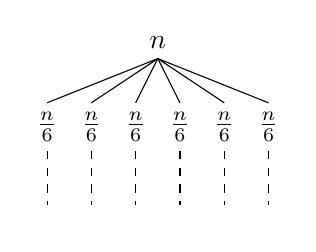
\begin{tikzpicture}
                    \Tree
                    [.$n$
                        [.$\frac{n}{6}$
                            \edge[dashed];
                            [.$$
                            ]
                        ]
                        [.$\frac{n}{6}$
                            \edge[dashed];
                            [.$$
                            ]
                        ]
                        [.$\frac{n}{6}$
                            \edge[dashed];
                            [.$$
                            ]
                        ]
                        [.$\frac{n}{6}$
                            \edge[dashed];
                            [.$$
                            ]
                        ]
                        [.$\frac{n}{6}$
                            \edge[dashed];
                            [.$$
                            ]
                        ]
                        [.$\frac{n}{6}$
                            \edge[dashed];
                            [.$$
                            ]
                        ]
                    ]     
                \end{tikzpicture} \\
            \end{center}
            \begin{center}
                At level $k^{th}$ level we are doing $\frac{6^kn}{6^k}$ work and there are $\log_6n$ levels...                
            \end{center}
            \begin{align*}
                \sum_{k=0}^{\log_6n} \left(\frac{\cancel{6^k}n}{\cancel{6^k}}\right) &= n\sum_{k=0}^{\log_6n}1\\
                &= n \log_6(n) \\
                &= \boxed{\Theta\left(n\log n\right)} \\
            \end{align*}
        \newpage
        \color{black}
        \item[\textbf{(e)}] $T(n) = T(3n/5) + T(4n/5) (\text{We have } T(1) = 1)$ \\
        \color{blue}
            \begin{center}
                We can try finding an upper and lower bound for $T(n)$:
            \end{center}
            \begin{align*}
                \text{UPPER: } T(n) &\le 2T(4n/5) \\
                \text{LOWER: } T(n) &\ge 2T(3n/5)
            \end{align*}
            \begin{center}
                We can use Masters Theorem to solve the two realtions..
            \end{center}
            \begin{align*}
                \text{UPPER: } &a = 2, b = \frac{5}{4}, d = 0 \\
                &\log_{\frac{5}{4}}2 > d = 0\\
                &\therefore \mathcal{O}(n^{\log_{\frac{5}{4}}2}) \approx \mathcal{O}(n^{3.11})\\
                \text{LOWER: } &a = 2, b = \frac{5}{3}, d = 0 \\
                &\log_{\frac{5}{3}}2 > d = 0\\
                &\therefore \Omega(n^{\log_{\frac{5}{3}}2}) \approx \Omega(n^{1.36})
            \end{align*}
            \begin{align*}
                T(n) &= an^b, T(1) = 1 \\
                T(1) &= a1^b = a = 1
            \end{align*}
            \begin{center}
                Plug in $n=an^b$ into $T(n)$ with $a = 1$
            \end{center}
            \begin{align*}
                n^b &= \left(\frac{3n}{5}\right)^b + \left(\frac{4n}{5}\right)^b \\
                n^b &= \left(\frac{3^b}{5^b}\right)n^b + \left(\frac{4^b}{5^b}\right)n^b \\
                1 &= \frac{3^b + 4^b}{5^b} \\
                5^b &= 3^b + 4^b \\
                b &= 2, \text{ since } 9 + 16 = 25 \\
                &\boxed{\Theta(n^2)}
            \end{align*}
    \end{enumerate}
    \newpage
    \section*{6 In Between Functions}
    \begin{enumerate}
        \item[\textbf{(a)}] Try setting $f(n)$ to a polynomial of degree d, where d is a very large constant. So
        $f(n) = a_0 + a_1n + a_2n^2 + \cdots + a_dn^d$. For which values of k (if any) does f fail to satisfy (1)?\\
        \color{blue}
        \begin{center}
            Since the last term dominates, in order for (1) to not be satisfied then $d\ge k$, and/or $a$ would have to a large value such that $a_dn^d \ge n^k$.
        \end{center}
        \color{black}
        \item[\textbf{(b)}] Now try setting $f(n)$ to $a^n$, for some constant $a > 1$ that’s as small as possible while
        still satisfying (1) (e.g. 1.000001). For which values of $c$ (if any) does $f$ fail to satisfy (2)?
        \color{blue}
            \begin{center}
                $f(n) = a^n, a > 1$ \\
                Let $a = 2^b \Rightarrow b = log_2(a), f(n) = 2^{bn}$
                \begin{align*}
                    2^{bn} &\ge 2^{cn} \\
                    b &\ge c \\
                    log_2(a) &\ge c
                \end{align*}
                In order for (2) to not be satisfied, $b=log_2(a)$ would have to be greater than $c$.
            \end{center}
        \color{black}
        \item[\textbf{(c)}] Find a function $D(n)$ such that setting $f(n) = O(nD(n))$ satisfies both (1) and (2). Give   
        a proof that your answer satisfies both.\\
        \color{blue}
        \begin{center}
            Let $D(n) = log(n)$ \\
            $f(n) = O(n^{log n})$ 
        \end{center}
        \begin{align*}
            \begin{split}
                n^{\log n} &> n^k\\
                \log n &> k \textbf{ (i)}
            \end{split}
            \begin{split}
                n^{\log n} &< 2^{cn} \\
                \log(n^{\log n}) &< \log(2^{cn}) \\
                \log n \log n &< cn\log 2\\
                \log^2n &< cn\log 2 \textbf{ (ii)}
            \end{split}
        \end{align*}
        \begin{center}
            Since $\log n$ is greater than any constant k, \textbf{(i)} satisfies (1). Similarly $\log^2 n$ is less than $cn \log 2$ \textbf{(ii)} satisfying (2).
        \end{center}
    \end{enumerate}
    \newpage
\end{document}